% !TEX encoding = UTF-8 Unicode
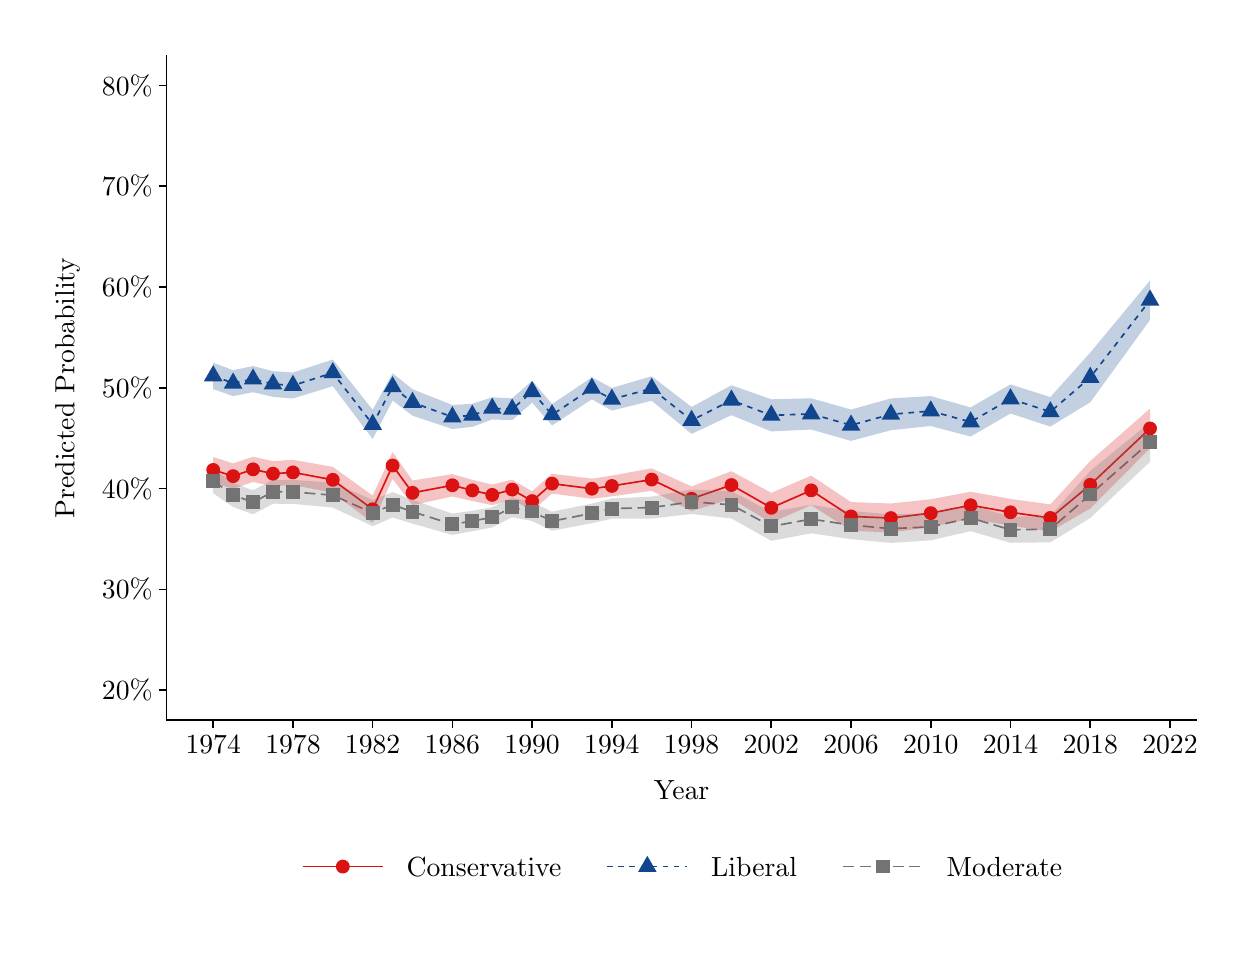
\begin{tikzpicture}[x=1pt,y=1pt]
\definecolor{fillColor}{RGB}{255,255,255}
\path[use as bounding box,fill=fillColor,fill opacity=0.00] (0,0) rectangle (432.48,324.36);
\begin{scope}
\path[clip] (  0.00,  0.00) rectangle (432.48,324.36);
\definecolor{fillColor}{RGB}{255,255,255}

\path[fill=fillColor] ( -0.00,  0.00) rectangle (432.48,324.36);
\end{scope}
\begin{scope}
\path[clip] ( 50.11, 74.07) rectangle (422.48,314.36);
\definecolor{fillColor}{RGB}{255,255,255}

\path[fill=fillColor] ( 50.11, 74.07) rectangle (422.48,314.36);
\definecolor{drawColor}{RGB}{218,18,18}

\path[draw=drawColor,line width= 0.6pt,line join=round] ( 67.04,164.55) --
	( 74.24,162.30) --
	( 81.44,164.76) --
	( 88.64,163.19) --
	( 95.85,163.66) --
	(110.25,160.97) --
	(124.66,150.33) --
	(131.86,166.14) --
	(139.06,156.27) --
	(153.47,159.00) --
	(160.67,157.16) --
	(167.87,155.52) --
	(175.07,157.44) --
	(182.28,153.29) --
	(189.48,159.60) --
	(203.88,157.76) --
	(211.09,158.76) --
	(225.49,161.06) --
	(239.90,154.13) --
	(254.30,159.09) --
	(268.71,150.86) --
	(283.11,157.17) --
	(297.52,147.75) --
	(311.92,147.16) --
	(326.33,148.94) --
	(340.73,151.78) --
	(355.14,149.24) --
	(369.54,147.20) --
	(383.95,159.17) --
	(405.56,179.53);
\definecolor{drawColor}{RGB}{17,70,143}

\path[draw=drawColor,line width= 0.6pt,dash pattern=on 2pt off 2pt ,line join=round] ( 67.04,198.53) --
	( 74.24,195.90) --
	( 81.44,197.36) --
	( 88.64,195.59) --
	( 95.85,195.05) --
	(110.25,199.63) --
	(124.66,181.00) --
	(131.86,194.56) --
	(139.06,188.93) --
	(153.47,183.68) --
	(160.67,184.29) --
	(167.87,186.80) --
	(175.07,186.48) --
	(182.28,192.83) --
	(189.48,184.47) --
	(203.88,194.05) --
	(211.09,190.09) --
	(225.49,193.96) --
	(239.90,182.43) --
	(254.30,189.75) --
	(268.71,184.26) --
	(283.11,184.80) --
	(297.52,180.71) --
	(311.92,184.64) --
	(326.33,185.83) --
	(340.73,181.87) --
	(355.14,190.21) --
	(369.54,185.54) --
	(383.95,197.96) --
	(405.56,225.88);
\definecolor{drawColor}{gray}{0.45}

\path[draw=drawColor,line width= 0.6pt,dash pattern=on 4pt off 2pt ,line join=round] ( 67.04,160.60) --
	( 74.24,155.49) --
	( 81.44,152.85) --
	( 88.64,156.67) --
	( 95.85,156.62) --
	(110.25,155.42) --
	(124.66,148.98) --
	(131.86,151.96) --
	(139.06,149.44) --
	(153.47,144.91) --
	(160.67,146.09) --
	(167.87,147.44) --
	(175.07,151.01) --
	(182.28,149.50) --
	(189.48,146.03) --
	(203.88,148.86) --
	(211.09,150.58) --
	(225.49,150.94) --
	(239.90,153.05) --
	(254.30,151.92) --
	(268.71,144.15) --
	(283.11,146.79) --
	(297.52,144.62) --
	(311.92,143.33) --
	(326.33,143.99) --
	(340.73,147.18) --
	(355.14,142.92) --
	(369.54,143.15) --
	(383.95,155.66) --
	(405.56,174.64);
\definecolor{fillColor}{RGB}{218,18,18}

\path[fill=fillColor,fill opacity=0.25] ( 67.04,169.24) --
	( 74.24,166.89) --
	( 81.44,169.32) --
	( 88.64,167.72) --
	( 95.85,168.21) --
	(110.25,165.65) --
	(124.66,155.26) --
	(131.86,170.95) --
	(139.06,160.72) --
	(153.47,163.03) --
	(160.67,160.99) --
	(167.87,159.24) --
	(175.07,161.05) --
	(182.28,156.82) --
	(189.48,163.18) --
	(203.88,161.40) --
	(211.09,162.50) --
	(225.49,165.12) --
	(239.90,158.58) --
	(254.30,164.09) --
	(268.71,156.26) --
	(283.11,162.49) --
	(297.52,152.93) --
	(311.92,152.40) --
	(326.33,153.96) --
	(340.73,156.67) --
	(355.14,154.06) --
	(369.54,152.09) --
	(383.95,167.76) --
	(405.56,186.72) --
	(405.56,172.35) --
	(383.95,150.58) --
	(369.54,142.32) --
	(355.14,144.43) --
	(340.73,146.90) --
	(326.33,143.93) --
	(311.92,141.91) --
	(297.52,142.58) --
	(283.11,151.84) --
	(268.71,145.46) --
	(254.30,154.09) --
	(239.90,149.68) --
	(225.49,157.01) --
	(211.09,155.01) --
	(203.88,154.12) --
	(189.48,156.02) --
	(182.28,149.75) --
	(175.07,153.84) --
	(167.87,151.80) --
	(160.67,153.32) --
	(153.47,154.97) --
	(139.06,151.82) --
	(131.86,161.33) --
	(124.66,145.41) --
	(110.25,156.29) --
	( 95.85,159.11) --
	( 88.64,158.65) --
	( 81.44,160.20) --
	( 74.24,157.72) --
	( 67.04,159.86) --
	cycle;

\path[] ( 67.04,169.24) --
	( 74.24,166.89) --
	( 81.44,169.32) --
	( 88.64,167.72) --
	( 95.85,168.21) --
	(110.25,165.65) --
	(124.66,155.26) --
	(131.86,170.95) --
	(139.06,160.72) --
	(153.47,163.03) --
	(160.67,160.99) --
	(167.87,159.24) --
	(175.07,161.05) --
	(182.28,156.82) --
	(189.48,163.18) --
	(203.88,161.40) --
	(211.09,162.50) --
	(225.49,165.12) --
	(239.90,158.58) --
	(254.30,164.09) --
	(268.71,156.26) --
	(283.11,162.49) --
	(297.52,152.93) --
	(311.92,152.40) --
	(326.33,153.96) --
	(340.73,156.67) --
	(355.14,154.06) --
	(369.54,152.09) --
	(383.95,167.76) --
	(405.56,186.72);

\path[] (405.56,172.35) --
	(383.95,150.58) --
	(369.54,142.32) --
	(355.14,144.43) --
	(340.73,146.90) --
	(326.33,143.93) --
	(311.92,141.91) --
	(297.52,142.58) --
	(283.11,151.84) --
	(268.71,145.46) --
	(254.30,154.09) --
	(239.90,149.68) --
	(225.49,157.01) --
	(211.09,155.01) --
	(203.88,154.12) --
	(189.48,156.02) --
	(182.28,149.75) --
	(175.07,153.84) --
	(167.87,151.80) --
	(160.67,153.32) --
	(153.47,154.97) --
	(139.06,151.82) --
	(131.86,161.33) --
	(124.66,145.41) --
	(110.25,156.29) --
	( 95.85,159.11) --
	( 88.64,158.65) --
	( 81.44,160.20) --
	( 74.24,157.72) --
	( 67.04,159.86);
\definecolor{fillColor}{RGB}{17,70,143}

\path[fill=fillColor,fill opacity=0.25] ( 67.04,203.29) --
	( 74.24,200.57) --
	( 81.44,202.08) --
	( 88.64,200.23) --
	( 95.85,199.74) --
	(110.25,204.44) --
	(124.66,186.27) --
	(131.86,199.48) --
	(139.06,193.71) --
	(153.47,188.01) --
	(160.67,188.47) --
	(167.87,190.80) --
	(175.07,190.43) --
	(182.28,196.78) --
	(189.48,188.34) --
	(203.88,198.02) --
	(211.09,194.19) --
	(225.49,198.39) --
	(239.90,187.30) --
	(254.30,195.15) --
	(268.71,190.07) --
	(283.11,190.45) --
	(297.52,186.37) --
	(311.92,190.38) --
	(326.33,191.24) --
	(340.73,187.14) --
	(355.14,195.46) --
	(369.54,190.87) --
	(383.95,206.94) --
	(405.56,232.98) --
	(405.56,218.77) --
	(383.95,188.99) --
	(369.54,180.21) --
	(355.14,184.95) --
	(340.73,176.61) --
	(326.33,180.41) --
	(311.92,178.90) --
	(297.52,175.05) --
	(283.11,179.14) --
	(268.71,178.46) --
	(254.30,184.34) --
	(239.90,177.57) --
	(225.49,189.54) --
	(211.09,185.99) --
	(203.88,190.08) --
	(189.48,180.60) --
	(182.28,188.88) --
	(175.07,182.53) --
	(167.87,182.79) --
	(160.67,180.11) --
	(153.47,179.34) --
	(139.06,184.15) --
	(131.86,189.64) --
	(124.66,175.73) --
	(110.25,194.82) --
	( 95.85,190.36) --
	( 88.64,190.94) --
	( 81.44,192.64) --
	( 74.24,191.22) --
	( 67.04,193.77) --
	cycle;

\path[] ( 67.04,203.29) --
	( 74.24,200.57) --
	( 81.44,202.08) --
	( 88.64,200.23) --
	( 95.85,199.74) --
	(110.25,204.44) --
	(124.66,186.27) --
	(131.86,199.48) --
	(139.06,193.71) --
	(153.47,188.01) --
	(160.67,188.47) --
	(167.87,190.80) --
	(175.07,190.43) --
	(182.28,196.78) --
	(189.48,188.34) --
	(203.88,198.02) --
	(211.09,194.19) --
	(225.49,198.39) --
	(239.90,187.30) --
	(254.30,195.15) --
	(268.71,190.07) --
	(283.11,190.45) --
	(297.52,186.37) --
	(311.92,190.38) --
	(326.33,191.24) --
	(340.73,187.14) --
	(355.14,195.46) --
	(369.54,190.87) --
	(383.95,206.94) --
	(405.56,232.98);

\path[] (405.56,218.77) --
	(383.95,188.99) --
	(369.54,180.21) --
	(355.14,184.95) --
	(340.73,176.61) --
	(326.33,180.41) --
	(311.92,178.90) --
	(297.52,175.05) --
	(283.11,179.14) --
	(268.71,178.46) --
	(254.30,184.34) --
	(239.90,177.57) --
	(225.49,189.54) --
	(211.09,185.99) --
	(203.88,190.08) --
	(189.48,180.60) --
	(182.28,188.88) --
	(175.07,182.53) --
	(167.87,182.79) --
	(160.67,180.11) --
	(153.47,179.34) --
	(139.06,184.15) --
	(131.86,189.64) --
	(124.66,175.73) --
	(110.25,194.82) --
	( 95.85,190.36) --
	( 88.64,190.94) --
	( 81.44,192.64) --
	( 74.24,191.22) --
	( 67.04,193.77);
\definecolor{fillColor}{RGB}{115,115,115}

\path[fill=fillColor,fill opacity=0.25] ( 67.04,165.06) --
	( 74.24,159.84) --
	( 81.44,157.18) --
	( 88.64,160.99) --
	( 95.85,160.95) --
	(110.25,159.91) --
	(124.66,153.73) --
	(131.86,156.56) --
	(139.06,153.72) --
	(153.47,148.76) --
	(160.67,149.77) --
	(167.87,151.07) --
	(175.07,154.56) --
	(182.28,152.93) --
	(189.48,149.47) --
	(203.88,152.40) --
	(211.09,154.24) --
	(225.49,154.90) --
	(239.90,157.47) --
	(254.30,156.84) --
	(268.71,149.38) --
	(283.11,151.92) --
	(297.52,149.70) --
	(311.92,148.50) --
	(326.33,148.85) --
	(340.73,151.94) --
	(355.14,147.61) --
	(369.54,147.93) --
	(383.95,164.16) --
	(405.56,181.80) --
	(405.56,167.47) --
	(383.95,147.17) --
	(369.54,138.37) --
	(355.14,138.23) --
	(340.73,142.42) --
	(326.33,139.13) --
	(311.92,138.17) --
	(297.52,139.54) --
	(283.11,141.65) --
	(268.71,138.92) --
	(254.30,147.01) --
	(239.90,148.62) --
	(225.49,146.98) --
	(211.09,146.92) --
	(203.88,145.32) --
	(189.48,142.60) --
	(182.28,146.08) --
	(175.07,147.47) --
	(167.87,143.80) --
	(160.67,142.40) --
	(153.47,141.06) --
	(139.06,145.16) --
	(131.86,147.36) --
	(124.66,144.23) --
	(110.25,150.94) --
	( 95.85,152.29) --
	( 88.64,152.34) --
	( 81.44,148.52) --
	( 74.24,151.13) --
	( 67.04,156.13) --
	cycle;

\path[] ( 67.04,165.06) --
	( 74.24,159.84) --
	( 81.44,157.18) --
	( 88.64,160.99) --
	( 95.85,160.95) --
	(110.25,159.91) --
	(124.66,153.73) --
	(131.86,156.56) --
	(139.06,153.72) --
	(153.47,148.76) --
	(160.67,149.77) --
	(167.87,151.07) --
	(175.07,154.56) --
	(182.28,152.93) --
	(189.48,149.47) --
	(203.88,152.40) --
	(211.09,154.24) --
	(225.49,154.90) --
	(239.90,157.47) --
	(254.30,156.84) --
	(268.71,149.38) --
	(283.11,151.92) --
	(297.52,149.70) --
	(311.92,148.50) --
	(326.33,148.85) --
	(340.73,151.94) --
	(355.14,147.61) --
	(369.54,147.93) --
	(383.95,164.16) --
	(405.56,181.80);

\path[] (405.56,167.47) --
	(383.95,147.17) --
	(369.54,138.37) --
	(355.14,138.23) --
	(340.73,142.42) --
	(326.33,139.13) --
	(311.92,138.17) --
	(297.52,139.54) --
	(283.11,141.65) --
	(268.71,138.92) --
	(254.30,147.01) --
	(239.90,148.62) --
	(225.49,146.98) --
	(211.09,146.92) --
	(203.88,145.32) --
	(189.48,142.60) --
	(182.28,146.08) --
	(175.07,147.47) --
	(167.87,143.80) --
	(160.67,142.40) --
	(153.47,141.06) --
	(139.06,145.16) --
	(131.86,147.36) --
	(124.66,144.23) --
	(110.25,150.94) --
	( 95.85,152.29) --
	( 88.64,152.34) --
	( 81.44,148.52) --
	( 74.24,151.13) --
	( 67.04,156.13);
\definecolor{fillColor}{RGB}{17,70,143}

\path[fill=fillColor] ( 67.04,202.42) --
	( 70.40,196.59) --
	( 63.67,196.59) --
	cycle;

\path[fill=fillColor] ( 74.24,199.78) --
	( 77.60,193.95) --
	( 70.87,193.95) --
	cycle;

\path[fill=fillColor] ( 81.44,201.25) --
	( 84.80,195.42) --
	( 78.08,195.42) --
	cycle;

\path[fill=fillColor] ( 88.64,199.47) --
	( 92.01,193.64) --
	( 85.28,193.64) --
	cycle;

\path[fill=fillColor] ( 95.85,198.94) --
	( 99.21,193.11) --
	( 92.48,193.11) --
	cycle;

\path[fill=fillColor] (110.25,203.52) --
	(113.62,197.69) --
	(106.89,197.69) --
	cycle;

\path[fill=fillColor] (124.66,184.88) --
	(128.02,179.06) --
	(121.29,179.06) --
	cycle;

\path[fill=fillColor] (131.86,198.44) --
	(135.22,192.62) --
	(128.50,192.62) --
	cycle;

\path[fill=fillColor] (139.06,192.81) --
	(142.43,186.99) --
	(135.70,186.99) --
	cycle;

\path[fill=fillColor] (153.47,187.56) --
	(156.83,181.73) --
	(150.10,181.73) --
	cycle;

\path[fill=fillColor] (160.67,188.17) --
	(164.03,182.35) --
	(157.31,182.35) --
	cycle;

\path[fill=fillColor] (167.87,190.68) --
	(171.24,184.85) --
	(164.51,184.85) --
	cycle;

\path[fill=fillColor] (175.07,190.36) --
	(178.44,184.54) --
	(171.71,184.54) --
	cycle;

\path[fill=fillColor] (182.28,196.71) --
	(185.64,190.89) --
	(178.91,190.89) --
	cycle;

\path[fill=fillColor] (189.48,188.35) --
	(192.84,182.53) --
	(186.12,182.53) --
	cycle;

\path[fill=fillColor] (203.88,197.93) --
	(207.25,192.11) --
	(200.52,192.11) --
	cycle;

\path[fill=fillColor] (211.09,193.97) --
	(214.45,188.14) --
	(207.72,188.14) --
	cycle;

\path[fill=fillColor] (225.49,197.85) --
	(228.86,192.02) --
	(222.13,192.02) --
	cycle;

\path[fill=fillColor] (239.90,186.32) --
	(243.26,180.49) --
	(236.53,180.49) --
	cycle;

\path[fill=fillColor] (254.30,193.63) --
	(257.67,187.81) --
	(250.94,187.81) --
	cycle;

\path[fill=fillColor] (268.71,188.15) --
	(272.07,182.32) --
	(265.34,182.32) --
	cycle;

\path[fill=fillColor] (283.11,188.68) --
	(286.48,182.85) --
	(279.75,182.85) --
	cycle;

\path[fill=fillColor] (297.52,184.59) --
	(300.88,178.77) --
	(294.15,178.77) --
	cycle;

\path[fill=fillColor] (311.92,188.52) --
	(315.29,182.70) --
	(308.56,182.70) --
	cycle;

\path[fill=fillColor] (326.33,189.71) --
	(329.69,183.89) --
	(322.96,183.89) --
	cycle;

\path[fill=fillColor] (340.73,185.76) --
	(344.10,179.93) --
	(337.37,179.93) --
	cycle;

\path[fill=fillColor] (355.14,194.09) --
	(358.50,188.27) --
	(351.77,188.27) --
	cycle;

\path[fill=fillColor] (369.54,189.42) --
	(372.91,183.60) --
	(366.18,183.60) --
	cycle;

\path[fill=fillColor] (383.95,201.85) --
	(387.31,196.02) --
	(380.58,196.02) --
	cycle;

\path[fill=fillColor] (405.56,229.76) --
	(408.92,223.93) --
	(402.19,223.93) --
	cycle;
\definecolor{fillColor}{RGB}{218,18,18}

\path[fill=fillColor] ( 67.04,164.55) circle (  2.50);

\path[fill=fillColor] ( 74.24,162.30) circle (  2.50);

\path[fill=fillColor] ( 81.44,164.76) circle (  2.50);

\path[fill=fillColor] ( 88.64,163.19) circle (  2.50);

\path[fill=fillColor] ( 95.85,163.66) circle (  2.50);

\path[fill=fillColor] (110.25,160.97) circle (  2.50);

\path[fill=fillColor] (124.66,150.33) circle (  2.50);

\path[fill=fillColor] (131.86,166.14) circle (  2.50);

\path[fill=fillColor] (139.06,156.27) circle (  2.50);

\path[fill=fillColor] (153.47,159.00) circle (  2.50);

\path[fill=fillColor] (160.67,157.16) circle (  2.50);

\path[fill=fillColor] (167.87,155.52) circle (  2.50);

\path[fill=fillColor] (175.07,157.44) circle (  2.50);

\path[fill=fillColor] (182.28,153.29) circle (  2.50);

\path[fill=fillColor] (189.48,159.60) circle (  2.50);

\path[fill=fillColor] (203.88,157.76) circle (  2.50);

\path[fill=fillColor] (211.09,158.76) circle (  2.50);

\path[fill=fillColor] (225.49,161.06) circle (  2.50);

\path[fill=fillColor] (239.90,154.13) circle (  2.50);

\path[fill=fillColor] (254.30,159.09) circle (  2.50);

\path[fill=fillColor] (268.71,150.86) circle (  2.50);

\path[fill=fillColor] (283.11,157.17) circle (  2.50);

\path[fill=fillColor] (297.52,147.75) circle (  2.50);

\path[fill=fillColor] (311.92,147.16) circle (  2.50);

\path[fill=fillColor] (326.33,148.94) circle (  2.50);

\path[fill=fillColor] (340.73,151.78) circle (  2.50);

\path[fill=fillColor] (355.14,149.24) circle (  2.50);

\path[fill=fillColor] (369.54,147.20) circle (  2.50);

\path[fill=fillColor] (383.95,159.17) circle (  2.50);

\path[fill=fillColor] (405.56,179.53) circle (  2.50);
\definecolor{fillColor}{gray}{0.45}

\path[fill=fillColor] ( 64.54,158.10) --
	( 69.53,158.10) --
	( 69.53,163.09) --
	( 64.54,163.09) --
	cycle;

\path[fill=fillColor] ( 71.74,152.99) --
	( 76.74,152.99) --
	( 76.74,157.98) --
	( 71.74,157.98) --
	cycle;

\path[fill=fillColor] ( 78.94,150.35) --
	( 83.94,150.35) --
	( 83.94,155.35) --
	( 78.94,155.35) --
	cycle;

\path[fill=fillColor] ( 86.15,154.17) --
	( 91.14,154.17) --
	( 91.14,159.16) --
	( 86.15,159.16) --
	cycle;

\path[fill=fillColor] ( 93.35,154.12) --
	( 98.34,154.12) --
	( 98.34,159.12) --
	( 93.35,159.12) --
	cycle;

\path[fill=fillColor] (107.75,152.92) --
	(112.75,152.92) --
	(112.75,157.92) --
	(107.75,157.92) --
	cycle;

\path[fill=fillColor] (122.16,146.48) --
	(127.15,146.48) --
	(127.15,151.48) --
	(122.16,151.48) --
	cycle;

\path[fill=fillColor] (129.36,149.46) --
	(134.36,149.46) --
	(134.36,154.46) --
	(129.36,154.46) --
	cycle;

\path[fill=fillColor] (136.56,146.94) --
	(141.56,146.94) --
	(141.56,151.94) --
	(136.56,151.94) --
	cycle;

\path[fill=fillColor] (150.97,142.41) --
	(155.96,142.41) --
	(155.96,147.41) --
	(150.97,147.41) --
	cycle;

\path[fill=fillColor] (158.17,143.59) --
	(163.17,143.59) --
	(163.17,148.59) --
	(158.17,148.59) --
	cycle;

\path[fill=fillColor] (165.37,144.94) --
	(170.37,144.94) --
	(170.37,149.93) --
	(165.37,149.93) --
	cycle;

\path[fill=fillColor] (172.58,148.52) --
	(177.57,148.52) --
	(177.57,153.51) --
	(172.58,153.51) --
	cycle;

\path[fill=fillColor] (179.78,147.01) --
	(184.77,147.01) --
	(184.77,152.00) --
	(179.78,152.00) --
	cycle;

\path[fill=fillColor] (186.98,143.53) --
	(191.98,143.53) --
	(191.98,148.53) --
	(186.98,148.53) --
	cycle;

\path[fill=fillColor] (201.39,146.36) --
	(206.38,146.36) --
	(206.38,151.36) --
	(201.39,151.36) --
	cycle;

\path[fill=fillColor] (208.59,148.08) --
	(213.58,148.08) --
	(213.58,153.08) --
	(208.59,153.08) --
	cycle;

\path[fill=fillColor] (222.99,148.44) --
	(227.99,148.44) --
	(227.99,153.44) --
	(222.99,153.44) --
	cycle;

\path[fill=fillColor] (237.40,150.55) --
	(242.39,150.55) --
	(242.39,155.54) --
	(237.40,155.54) --
	cycle;

\path[fill=fillColor] (251.80,149.43) --
	(256.80,149.43) --
	(256.80,154.42) --
	(251.80,154.42) --
	cycle;

\path[fill=fillColor] (266.21,141.65) --
	(271.21,141.65) --
	(271.21,146.65) --
	(266.21,146.65) --
	cycle;

\path[fill=fillColor] (280.61,144.29) --
	(285.61,144.29) --
	(285.61,149.28) --
	(280.61,149.28) --
	cycle;

\path[fill=fillColor] (295.02,142.12) --
	(300.02,142.12) --
	(300.02,147.12) --
	(295.02,147.12) --
	cycle;

\path[fill=fillColor] (309.43,140.83) --
	(314.42,140.83) --
	(314.42,145.83) --
	(309.43,145.83) --
	cycle;

\path[fill=fillColor] (323.83,141.49) --
	(328.83,141.49) --
	(328.83,146.49) --
	(323.83,146.49) --
	cycle;

\path[fill=fillColor] (338.24,144.68) --
	(343.23,144.68) --
	(343.23,149.68) --
	(338.24,149.68) --
	cycle;

\path[fill=fillColor] (352.64,140.42) --
	(357.64,140.42) --
	(357.64,145.42) --
	(352.64,145.42) --
	cycle;

\path[fill=fillColor] (367.05,140.65) --
	(372.04,140.65) --
	(372.04,145.65) --
	(367.05,145.65) --
	cycle;

\path[fill=fillColor] (381.45,153.17) --
	(386.45,153.17) --
	(386.45,158.16) --
	(381.45,158.16) --
	cycle;

\path[fill=fillColor] (403.06,172.14) --
	(408.05,172.14) --
	(408.05,177.13) --
	(403.06,177.13) --
	cycle;
\end{scope}
\begin{scope}
\path[clip] (  0.00,  0.00) rectangle (432.48,324.36);
\definecolor{drawColor}{RGB}{0,0,0}

\path[draw=drawColor,line width= 0.6pt,line join=round] ( 50.11, 74.07) --
	( 50.11,314.36);
\end{scope}
\begin{scope}
\path[clip] (  0.00,  0.00) rectangle (432.48,324.36);
\definecolor{drawColor}{RGB}{0,0,0}

\node[text=drawColor,anchor=base east,inner sep=0pt, outer sep=0pt, scale=  1.00] at ( 45.16, 81.55) {20{\%}};

\node[text=drawColor,anchor=base east,inner sep=0pt, outer sep=0pt, scale=  1.00] at ( 45.16,117.95) {30{\%}};

\node[text=drawColor,anchor=base east,inner sep=0pt, outer sep=0pt, scale=  1.00] at ( 45.16,154.36) {40{\%}};

\node[text=drawColor,anchor=base east,inner sep=0pt, outer sep=0pt, scale=  1.00] at ( 45.16,190.77) {50{\%}};

\node[text=drawColor,anchor=base east,inner sep=0pt, outer sep=0pt, scale=  1.00] at ( 45.16,227.18) {60{\%}};

\node[text=drawColor,anchor=base east,inner sep=0pt, outer sep=0pt, scale=  1.00] at ( 45.16,263.59) {70{\%}};

\node[text=drawColor,anchor=base east,inner sep=0pt, outer sep=0pt, scale=  1.00] at ( 45.16,300.00) {80{\%}};
\end{scope}
\begin{scope}
\path[clip] (  0.00,  0.00) rectangle (432.48,324.36);
\definecolor{drawColor}{RGB}{0,0,0}

\path[draw=drawColor,line width= 0.6pt,line join=round] ( 47.36, 84.99) --
	( 50.11, 84.99);

\path[draw=drawColor,line width= 0.6pt,line join=round] ( 47.36,121.40) --
	( 50.11,121.40);

\path[draw=drawColor,line width= 0.6pt,line join=round] ( 47.36,157.81) --
	( 50.11,157.81);

\path[draw=drawColor,line width= 0.6pt,line join=round] ( 47.36,194.21) --
	( 50.11,194.21);

\path[draw=drawColor,line width= 0.6pt,line join=round] ( 47.36,230.62) --
	( 50.11,230.62);

\path[draw=drawColor,line width= 0.6pt,line join=round] ( 47.36,267.03) --
	( 50.11,267.03);

\path[draw=drawColor,line width= 0.6pt,line join=round] ( 47.36,303.44) --
	( 50.11,303.44);
\end{scope}
\begin{scope}
\path[clip] (  0.00,  0.00) rectangle (432.48,324.36);
\definecolor{drawColor}{RGB}{0,0,0}

\path[draw=drawColor,line width= 0.6pt,line join=round] ( 50.11, 74.07) --
	(422.48, 74.07);
\end{scope}
\begin{scope}
\path[clip] (  0.00,  0.00) rectangle (432.48,324.36);
\definecolor{drawColor}{RGB}{0,0,0}

\path[draw=drawColor,line width= 0.6pt,line join=round] ( 67.04, 71.32) --
	( 67.04, 74.07);

\path[draw=drawColor,line width= 0.6pt,line join=round] ( 95.85, 71.32) --
	( 95.85, 74.07);

\path[draw=drawColor,line width= 0.6pt,line join=round] (124.66, 71.32) --
	(124.66, 74.07);

\path[draw=drawColor,line width= 0.6pt,line join=round] (153.47, 71.32) --
	(153.47, 74.07);

\path[draw=drawColor,line width= 0.6pt,line join=round] (182.28, 71.32) --
	(182.28, 74.07);

\path[draw=drawColor,line width= 0.6pt,line join=round] (211.09, 71.32) --
	(211.09, 74.07);

\path[draw=drawColor,line width= 0.6pt,line join=round] (239.90, 71.32) --
	(239.90, 74.07);

\path[draw=drawColor,line width= 0.6pt,line join=round] (268.71, 71.32) --
	(268.71, 74.07);

\path[draw=drawColor,line width= 0.6pt,line join=round] (297.52, 71.32) --
	(297.52, 74.07);

\path[draw=drawColor,line width= 0.6pt,line join=round] (326.33, 71.32) --
	(326.33, 74.07);

\path[draw=drawColor,line width= 0.6pt,line join=round] (355.14, 71.32) --
	(355.14, 74.07);

\path[draw=drawColor,line width= 0.6pt,line join=round] (383.95, 71.32) --
	(383.95, 74.07);

\path[draw=drawColor,line width= 0.6pt,line join=round] (412.76, 71.32) --
	(412.76, 74.07);
\end{scope}
\begin{scope}
\path[clip] (  0.00,  0.00) rectangle (432.48,324.36);
\definecolor{drawColor}{RGB}{0,0,0}

\node[text=drawColor,anchor=base,inner sep=0pt, outer sep=0pt, scale=  1.00] at ( 67.04, 62.23) {1974};

\node[text=drawColor,anchor=base,inner sep=0pt, outer sep=0pt, scale=  1.00] at ( 95.85, 62.23) {1978};

\node[text=drawColor,anchor=base,inner sep=0pt, outer sep=0pt, scale=  1.00] at (124.66, 62.23) {1982};

\node[text=drawColor,anchor=base,inner sep=0pt, outer sep=0pt, scale=  1.00] at (153.47, 62.23) {1986};

\node[text=drawColor,anchor=base,inner sep=0pt, outer sep=0pt, scale=  1.00] at (182.28, 62.23) {1990};

\node[text=drawColor,anchor=base,inner sep=0pt, outer sep=0pt, scale=  1.00] at (211.09, 62.23) {1994};

\node[text=drawColor,anchor=base,inner sep=0pt, outer sep=0pt, scale=  1.00] at (239.90, 62.23) {1998};

\node[text=drawColor,anchor=base,inner sep=0pt, outer sep=0pt, scale=  1.00] at (268.71, 62.23) {2002};

\node[text=drawColor,anchor=base,inner sep=0pt, outer sep=0pt, scale=  1.00] at (297.52, 62.23) {2006};

\node[text=drawColor,anchor=base,inner sep=0pt, outer sep=0pt, scale=  1.00] at (326.33, 62.23) {2010};

\node[text=drawColor,anchor=base,inner sep=0pt, outer sep=0pt, scale=  1.00] at (355.14, 62.23) {2014};

\node[text=drawColor,anchor=base,inner sep=0pt, outer sep=0pt, scale=  1.00] at (383.95, 62.23) {2018};

\node[text=drawColor,anchor=base,inner sep=0pt, outer sep=0pt, scale=  1.00] at (412.76, 62.23) {2022};
\end{scope}
\begin{scope}
\path[clip] (  0.00,  0.00) rectangle (432.48,324.36);
\definecolor{drawColor}{RGB}{0,0,0}

\node[text=drawColor,anchor=base,inner sep=0pt, outer sep=0pt, scale=  1.00] at (236.30, 45.40) {Year};
\end{scope}
\begin{scope}
\path[clip] (  0.00,  0.00) rectangle (432.48,324.36);
\definecolor{drawColor}{RGB}{0,0,0}

\node[text=drawColor,rotate= 90.00,anchor=base,inner sep=0pt, outer sep=0pt, scale=  1.00] at ( 16.89,194.21) {Predicted Probability};
\end{scope}
\begin{scope}
\path[clip] (  0.00,  0.00) rectangle (432.48,324.36);

\path[] ( 86.80, 10.00) rectangle (385.79, 32.45);
\end{scope}
\begin{scope}
\path[clip] (  0.00,  0.00) rectangle (432.48,324.36);

\path[] ( 95.80, 14.00) rectangle (131.94, 28.45);
\end{scope}
\begin{scope}
\path[clip] (  0.00,  0.00) rectangle (432.48,324.36);
\definecolor{drawColor}{RGB}{218,18,18}

\path[draw=drawColor,line width= 0.6pt,line join=round] ( 99.42, 21.23) -- (128.33, 21.23);
\end{scope}
\begin{scope}
\path[clip] (  0.00,  0.00) rectangle (432.48,324.36);
\definecolor{fillColor}{RGB}{218,18,18}

\path[fill=fillColor] (113.87, 21.23) circle (  2.50);
\end{scope}
\begin{scope}
\path[clip] (  0.00,  0.00) rectangle (432.48,324.36);

\path[] (205.84, 14.00) rectangle (241.98, 28.45);
\end{scope}
\begin{scope}
\path[clip] (  0.00,  0.00) rectangle (432.48,324.36);
\definecolor{drawColor}{RGB}{17,70,143}

\path[draw=drawColor,line width= 0.6pt,dash pattern=on 2pt off 2pt ,line join=round] (209.46, 21.23) -- (238.36, 21.23);
\end{scope}
\begin{scope}
\path[clip] (  0.00,  0.00) rectangle (432.48,324.36);
\definecolor{fillColor}{RGB}{17,70,143}

\path[fill=fillColor] (223.91, 25.11) --
	(227.27, 19.28) --
	(220.55, 19.28) --
	cycle;
\end{scope}
\begin{scope}
\path[clip] (  0.00,  0.00) rectangle (432.48,324.36);

\path[] (290.97, 14.00) rectangle (327.10, 28.45);
\end{scope}
\begin{scope}
\path[clip] (  0.00,  0.00) rectangle (432.48,324.36);
\definecolor{drawColor}{gray}{0.45}

\path[draw=drawColor,line width= 0.6pt,dash pattern=on 4pt off 2pt ,line join=round] (294.58, 21.23) -- (323.49, 21.23);
\end{scope}
\begin{scope}
\path[clip] (  0.00,  0.00) rectangle (432.48,324.36);
\definecolor{fillColor}{gray}{0.45}

\path[fill=fillColor] (306.54, 18.73) --
	(311.53, 18.73) --
	(311.53, 23.72) --
	(306.54, 23.72) --
	cycle;
\end{scope}
\begin{scope}
\path[clip] (  0.00,  0.00) rectangle (432.48,324.36);
\definecolor{drawColor}{RGB}{0,0,0}

\node[text=drawColor,anchor=base west,inner sep=0pt, outer sep=0pt, scale=  1.00] at (136.94, 17.78) {Conservative};
\end{scope}
\begin{scope}
\path[clip] (  0.00,  0.00) rectangle (432.48,324.36);
\definecolor{drawColor}{RGB}{0,0,0}

\node[text=drawColor,anchor=base west,inner sep=0pt, outer sep=0pt, scale=  1.00] at (246.98, 17.78) {Liberal};
\end{scope}
\begin{scope}
\path[clip] (  0.00,  0.00) rectangle (432.48,324.36);
\definecolor{drawColor}{RGB}{0,0,0}

\node[text=drawColor,anchor=base west,inner sep=0pt, outer sep=0pt, scale=  1.00] at (332.10, 17.78) {Moderate};
\end{scope}
\end{tikzpicture}
